% GNUPLOT: LaTeX picture with Postscript
\begingroup
  \makeatletter
  \providecommand\color[2][]{%
    \GenericError{(gnuplot) \space\space\space\@spaces}{%
      Package color not loaded in conjunction with
      terminal option `colourtext'%
    }{See the gnuplot documentation for explanation.%
    }{Either use 'blacktext' in gnuplot or load the package
      color.sty in LaTeX.}%
    \renewcommand\color[2][]{}%
  }%
  \providecommand\includegraphics[2][]{%
    \GenericError{(gnuplot) \space\space\space\@spaces}{%
      Package graphicx or graphics not loaded%
    }{See the gnuplot documentation for explanation.%
    }{The gnuplot epslatex terminal needs graphicx.sty or graphics.sty.}%
    \renewcommand\includegraphics[2][]{}%
  }%
  \providecommand\rotatebox[2]{#2}%
  \@ifundefined{ifGPcolor}{%
    \newif\ifGPcolor
    \GPcolorfalse
  }{}%
  \@ifundefined{ifGPblacktext}{%
    \newif\ifGPblacktext
    \GPblacktexttrue
  }{}%
  % define a \g@addto@macro without @ in the name:
  \let\gplgaddtomacro\g@addto@macro
  % define empty templates for all commands taking text:
  \gdef\gplbacktext{}%
  \gdef\gplfronttext{}%
  \makeatother
  \ifGPblacktext
    % no textcolor at all
    \def\colorrgb#1{}%
    \def\colorgray#1{}%
  \else
    % gray or color?
    \ifGPcolor
      \def\colorrgb#1{\color[rgb]{#1}}%
      \def\colorgray#1{\color[gray]{#1}}%
      \expandafter\def\csname LTw\endcsname{\color{white}}%
      \expandafter\def\csname LTb\endcsname{\color{black}}%
      \expandafter\def\csname LTa\endcsname{\color{black}}%
      \expandafter\def\csname LT0\endcsname{\color[rgb]{1,0,0}}%
      \expandafter\def\csname LT1\endcsname{\color[rgb]{0,1,0}}%
      \expandafter\def\csname LT2\endcsname{\color[rgb]{0,0,1}}%
      \expandafter\def\csname LT3\endcsname{\color[rgb]{1,0,1}}%
      \expandafter\def\csname LT4\endcsname{\color[rgb]{0,1,1}}%
      \expandafter\def\csname LT5\endcsname{\color[rgb]{1,1,0}}%
      \expandafter\def\csname LT6\endcsname{\color[rgb]{0,0,0}}%
      \expandafter\def\csname LT7\endcsname{\color[rgb]{1,0.3,0}}%
      \expandafter\def\csname LT8\endcsname{\color[rgb]{0.5,0.5,0.5}}%
    \else
      % gray
      \def\colorrgb#1{\color{black}}%
      \def\colorgray#1{\color[gray]{#1}}%
      \expandafter\def\csname LTw\endcsname{\color{white}}%
      \expandafter\def\csname LTb\endcsname{\color{black}}%
      \expandafter\def\csname LTa\endcsname{\color{black}}%
      \expandafter\def\csname LT0\endcsname{\color{black}}%
      \expandafter\def\csname LT1\endcsname{\color{black}}%
      \expandafter\def\csname LT2\endcsname{\color{black}}%
      \expandafter\def\csname LT3\endcsname{\color{black}}%
      \expandafter\def\csname LT4\endcsname{\color{black}}%
      \expandafter\def\csname LT5\endcsname{\color{black}}%
      \expandafter\def\csname LT6\endcsname{\color{black}}%
      \expandafter\def\csname LT7\endcsname{\color{black}}%
      \expandafter\def\csname LT8\endcsname{\color{black}}%
    \fi
  \fi
  \setlength{\unitlength}{0.0500bp}%
  \begin{picture}(8502.00,14172.00)%
      \csname LTb\endcsname%
      \put(4251,13952){\makebox(0,0){\strut{}Sinusspannung für verschiedene Frequenzen}}%
    \gplgaddtomacro\gplbacktext{%
      \csname LTb\endcsname%
      \put(946,11168){\makebox(0,0)[r]{\strut{}-1}}%
      \put(946,11380){\makebox(0,0)[r]{\strut{}-0.8}}%
      \put(946,11593){\makebox(0,0)[r]{\strut{}-0.6}}%
      \put(946,11805){\makebox(0,0)[r]{\strut{}-0.4}}%
      \put(946,12017){\makebox(0,0)[r]{\strut{}-0.2}}%
      \put(946,12230){\makebox(0,0)[r]{\strut{} 0}}%
      \put(946,12442){\makebox(0,0)[r]{\strut{} 0.2}}%
      \put(946,12654){\makebox(0,0)[r]{\strut{} 0.4}}%
      \put(946,12866){\makebox(0,0)[r]{\strut{} 0.6}}%
      \put(946,13079){\makebox(0,0)[r]{\strut{} 0.8}}%
      \put(946,13291){\makebox(0,0)[r]{\strut{} 1}}%
      \put(1078,10948){\makebox(0,0){\strut{} 0}}%
      \put(1633,10948){\makebox(0,0){\strut{} 0.001}}%
      \put(2188,10948){\makebox(0,0){\strut{} 0.002}}%
      \put(2744,10948){\makebox(0,0){\strut{} 0.003}}%
      \put(3299,10948){\makebox(0,0){\strut{} 0.004}}%
      \put(3854,10948){\makebox(0,0){\strut{} 0.005}}%
      \put(176,12229){\rotatebox{-270}{\makebox(0,0){\strut{}$U \ [V]$}}}%
      \put(2466,10618){\makebox(0,0){\strut{}$t \ [s]$}}%
      \put(2466,13621){\makebox(0,0){\strut{}Zeitverlauf $f=8kHz$}}%
    }%
    \gplgaddtomacro\gplfronttext{%
    }%
    \gplgaddtomacro\gplbacktext{%
      \csname LTb\endcsname%
      \put(5197,11168){\makebox(0,0)[r]{\strut{} 0}}%
      \put(5197,11433){\makebox(0,0)[r]{\strut{} 0.1}}%
      \put(5197,11699){\makebox(0,0)[r]{\strut{} 0.2}}%
      \put(5197,11964){\makebox(0,0)[r]{\strut{} 0.3}}%
      \put(5197,12230){\makebox(0,0)[r]{\strut{} 0.4}}%
      \put(5197,12495){\makebox(0,0)[r]{\strut{} 0.5}}%
      \put(5197,12760){\makebox(0,0)[r]{\strut{} 0.6}}%
      \put(5197,13026){\makebox(0,0)[r]{\strut{} 0.7}}%
      \put(5197,13291){\makebox(0,0)[r]{\strut{} 0.8}}%
      \put(5329,10948){\makebox(0,0){\strut{} 0}}%
      \put(5884,10948){\makebox(0,0){\strut{} 1000}}%
      \put(6439,10948){\makebox(0,0){\strut{} 2000}}%
      \put(6995,10948){\makebox(0,0){\strut{} 3000}}%
      \put(7550,10948){\makebox(0,0){\strut{} 4000}}%
      \put(8105,10948){\makebox(0,0){\strut{} 5000}}%
      \put(4427,12229){\rotatebox{-270}{\makebox(0,0){\strut{}$F$}}}%
      \put(6717,10618){\makebox(0,0){\strut{}$f \ [Hz]$}}%
      \put(6717,13621){\makebox(0,0){\strut{}Frequenzspektrum $f=8kHz$}}%
    }%
    \gplgaddtomacro\gplfronttext{%
    }%
    \gplgaddtomacro\gplbacktext{%
      \csname LTb\endcsname%
      \put(946,7680){\makebox(0,0)[r]{\strut{}-1}}%
      \put(946,7892){\makebox(0,0)[r]{\strut{}-0.8}}%
      \put(946,8105){\makebox(0,0)[r]{\strut{}-0.6}}%
      \put(946,8317){\makebox(0,0)[r]{\strut{}-0.4}}%
      \put(946,8529){\makebox(0,0)[r]{\strut{}-0.2}}%
      \put(946,8742){\makebox(0,0)[r]{\strut{} 0}}%
      \put(946,8954){\makebox(0,0)[r]{\strut{} 0.2}}%
      \put(946,9166){\makebox(0,0)[r]{\strut{} 0.4}}%
      \put(946,9378){\makebox(0,0)[r]{\strut{} 0.6}}%
      \put(946,9591){\makebox(0,0)[r]{\strut{} 0.8}}%
      \put(946,9803){\makebox(0,0)[r]{\strut{} 1}}%
      \put(1078,7460){\makebox(0,0){\strut{} 0}}%
      \put(1633,7460){\makebox(0,0){\strut{} 0.001}}%
      \put(2188,7460){\makebox(0,0){\strut{} 0.002}}%
      \put(2744,7460){\makebox(0,0){\strut{} 0.003}}%
      \put(3299,7460){\makebox(0,0){\strut{} 0.004}}%
      \put(3854,7460){\makebox(0,0){\strut{} 0.005}}%
      \put(176,8741){\rotatebox{-270}{\makebox(0,0){\strut{}$U \ [V]$}}}%
      \put(2466,7130){\makebox(0,0){\strut{}$t \ [s]$}}%
      \put(2466,10133){\makebox(0,0){\strut{}Zeitverlauf $f=4kHz$}}%
    }%
    \gplgaddtomacro\gplfronttext{%
    }%
    \gplgaddtomacro\gplbacktext{%
      \csname LTb\endcsname%
      \put(5197,7680){\makebox(0,0)[r]{\strut{} 0}}%
      \put(5197,7945){\makebox(0,0)[r]{\strut{} 0.1}}%
      \put(5197,8211){\makebox(0,0)[r]{\strut{} 0.2}}%
      \put(5197,8476){\makebox(0,0)[r]{\strut{} 0.3}}%
      \put(5197,8742){\makebox(0,0)[r]{\strut{} 0.4}}%
      \put(5197,9007){\makebox(0,0)[r]{\strut{} 0.5}}%
      \put(5197,9272){\makebox(0,0)[r]{\strut{} 0.6}}%
      \put(5197,9538){\makebox(0,0)[r]{\strut{} 0.7}}%
      \put(5197,9803){\makebox(0,0)[r]{\strut{} 0.8}}%
      \put(5329,7460){\makebox(0,0){\strut{} 0}}%
      \put(5884,7460){\makebox(0,0){\strut{} 1000}}%
      \put(6439,7460){\makebox(0,0){\strut{} 2000}}%
      \put(6995,7460){\makebox(0,0){\strut{} 3000}}%
      \put(7550,7460){\makebox(0,0){\strut{} 4000}}%
      \put(8105,7460){\makebox(0,0){\strut{} 5000}}%
      \put(4427,8741){\rotatebox{-270}{\makebox(0,0){\strut{}$F$}}}%
      \put(6717,7130){\makebox(0,0){\strut{}$f \ [Hz]$}}%
      \put(6717,10133){\makebox(0,0){\strut{}Frequenzspektrum $f=4kHz$}}%
    }%
    \gplgaddtomacro\gplfronttext{%
    }%
    \gplgaddtomacro\gplbacktext{%
      \csname LTb\endcsname%
      \put(1342,4192){\makebox(0,0)[r]{\strut{} 0.9915}}%
      \put(1342,4546){\makebox(0,0)[r]{\strut{} 0.992}}%
      \put(1342,4900){\makebox(0,0)[r]{\strut{} 0.9925}}%
      \put(1342,5254){\makebox(0,0)[r]{\strut{} 0.993}}%
      \put(1342,5608){\makebox(0,0)[r]{\strut{} 0.9935}}%
      \put(1342,5962){\makebox(0,0)[r]{\strut{} 0.994}}%
      \put(1342,6316){\makebox(0,0)[r]{\strut{} 0.9945}}%
      \put(1474,3972){\makebox(0,0){\strut{} 0}}%
      \put(1950,3972){\makebox(0,0){\strut{} 0.002}}%
      \put(2426,3972){\makebox(0,0){\strut{} 0.004}}%
      \put(2902,3972){\makebox(0,0){\strut{} 0.006}}%
      \put(3378,3972){\makebox(0,0){\strut{} 0.008}}%
      \put(3854,3972){\makebox(0,0){\strut{} 0.01}}%
      \put(176,5254){\rotatebox{-270}{\makebox(0,0){\strut{}$U \ [V]$}}}%
      \put(2664,3642){\makebox(0,0){\strut{}$t \ [s]$}}%
      \put(2664,6646){\makebox(0,0){\strut{}Zeitverlauf $f=10kHz$}}%
    }%
    \gplgaddtomacro\gplfronttext{%
    }%
    \gplgaddtomacro\gplbacktext{%
      \csname LTb\endcsname%
      \put(5197,4192){\makebox(0,0)[r]{\strut{} 0}}%
      \put(5197,4404){\makebox(0,0)[r]{\strut{} 0.1}}%
      \put(5197,4617){\makebox(0,0)[r]{\strut{} 0.2}}%
      \put(5197,4829){\makebox(0,0)[r]{\strut{} 0.3}}%
      \put(5197,5042){\makebox(0,0)[r]{\strut{} 0.4}}%
      \put(5197,5254){\makebox(0,0)[r]{\strut{} 0.5}}%
      \put(5197,5466){\makebox(0,0)[r]{\strut{} 0.6}}%
      \put(5197,5679){\makebox(0,0)[r]{\strut{} 0.7}}%
      \put(5197,5891){\makebox(0,0)[r]{\strut{} 0.8}}%
      \put(5197,6104){\makebox(0,0)[r]{\strut{} 0.9}}%
      \put(5197,6316){\makebox(0,0)[r]{\strut{} 1}}%
      \put(5329,3972){\makebox(0,0){\strut{} 0}}%
      \put(5884,3972){\makebox(0,0){\strut{} 1000}}%
      \put(6439,3972){\makebox(0,0){\strut{} 2000}}%
      \put(6995,3972){\makebox(0,0){\strut{} 3000}}%
      \put(7550,3972){\makebox(0,0){\strut{} 4000}}%
      \put(8105,3972){\makebox(0,0){\strut{} 5000}}%
      \put(4427,5254){\rotatebox{-270}{\makebox(0,0){\strut{}$F$}}}%
      \put(6717,3642){\makebox(0,0){\strut{}$f \ [Hz]$}}%
      \put(6717,6646){\makebox(0,0){\strut{}Frequenzspektrum $f=10kHz$}}%
    }%
    \gplgaddtomacro\gplfronttext{%
    }%
    \gplgaddtomacro\gplbacktext{%
      \csname LTb\endcsname%
      \put(946,704){\makebox(0,0)[r]{\strut{}-0.4}}%
      \put(946,970){\makebox(0,0)[r]{\strut{}-0.3}}%
      \put(946,1235){\makebox(0,0)[r]{\strut{}-0.2}}%
      \put(946,1501){\makebox(0,0)[r]{\strut{}-0.1}}%
      \put(946,1766){\makebox(0,0)[r]{\strut{} 0}}%
      \put(946,2032){\makebox(0,0)[r]{\strut{} 0.1}}%
      \put(946,2297){\makebox(0,0)[r]{\strut{} 0.2}}%
      \put(946,2563){\makebox(0,0)[r]{\strut{} 0.3}}%
      \put(946,2828){\makebox(0,0)[r]{\strut{} 0.4}}%
      \put(1078,484){\makebox(0,0){\strut{} 0}}%
      \put(1633,484){\makebox(0,0){\strut{} 0.001}}%
      \put(2188,484){\makebox(0,0){\strut{} 0.002}}%
      \put(2744,484){\makebox(0,0){\strut{} 0.003}}%
      \put(3299,484){\makebox(0,0){\strut{} 0.004}}%
      \put(3854,484){\makebox(0,0){\strut{} 0.005}}%
      \put(176,1766){\rotatebox{-270}{\makebox(0,0){\strut{}$U \ [V]$}}}%
      \put(2466,154){\makebox(0,0){\strut{}$t \ [s]$}}%
      \put(2466,3158){\makebox(0,0){\strut{}Zeitverlauf $f=15kHz$}}%
    }%
    \gplgaddtomacro\gplfronttext{%
    }%
    \gplgaddtomacro\gplbacktext{%
      \csname LTb\endcsname%
      \put(5329,704){\makebox(0,0)[r]{\strut{} 0}}%
      \put(5329,1007){\makebox(0,0)[r]{\strut{} 0.05}}%
      \put(5329,1311){\makebox(0,0)[r]{\strut{} 0.1}}%
      \put(5329,1614){\makebox(0,0)[r]{\strut{} 0.15}}%
      \put(5329,1918){\makebox(0,0)[r]{\strut{} 0.2}}%
      \put(5329,2221){\makebox(0,0)[r]{\strut{} 0.25}}%
      \put(5329,2525){\makebox(0,0)[r]{\strut{} 0.3}}%
      \put(5329,2828){\makebox(0,0)[r]{\strut{} 0.35}}%
      \put(5461,484){\makebox(0,0){\strut{} 0}}%
      \put(5902,484){\makebox(0,0){\strut{} 1000}}%
      \put(6342,484){\makebox(0,0){\strut{} 2000}}%
      \put(6783,484){\makebox(0,0){\strut{} 3000}}%
      \put(7224,484){\makebox(0,0){\strut{} 4000}}%
      \put(7664,484){\makebox(0,0){\strut{} 5000}}%
      \put(8105,484){\makebox(0,0){\strut{} 6000}}%
      \put(4427,1766){\rotatebox{-270}{\makebox(0,0){\strut{}$F$}}}%
      \put(6783,154){\makebox(0,0){\strut{}$f \ [Hz]$}}%
      \put(6783,3158){\makebox(0,0){\strut{}Frequenzspektrum $f=15kHz$}}%
    }%
    \gplgaddtomacro\gplfronttext{%
    }%
    \gplbacktext
    \put(0,0){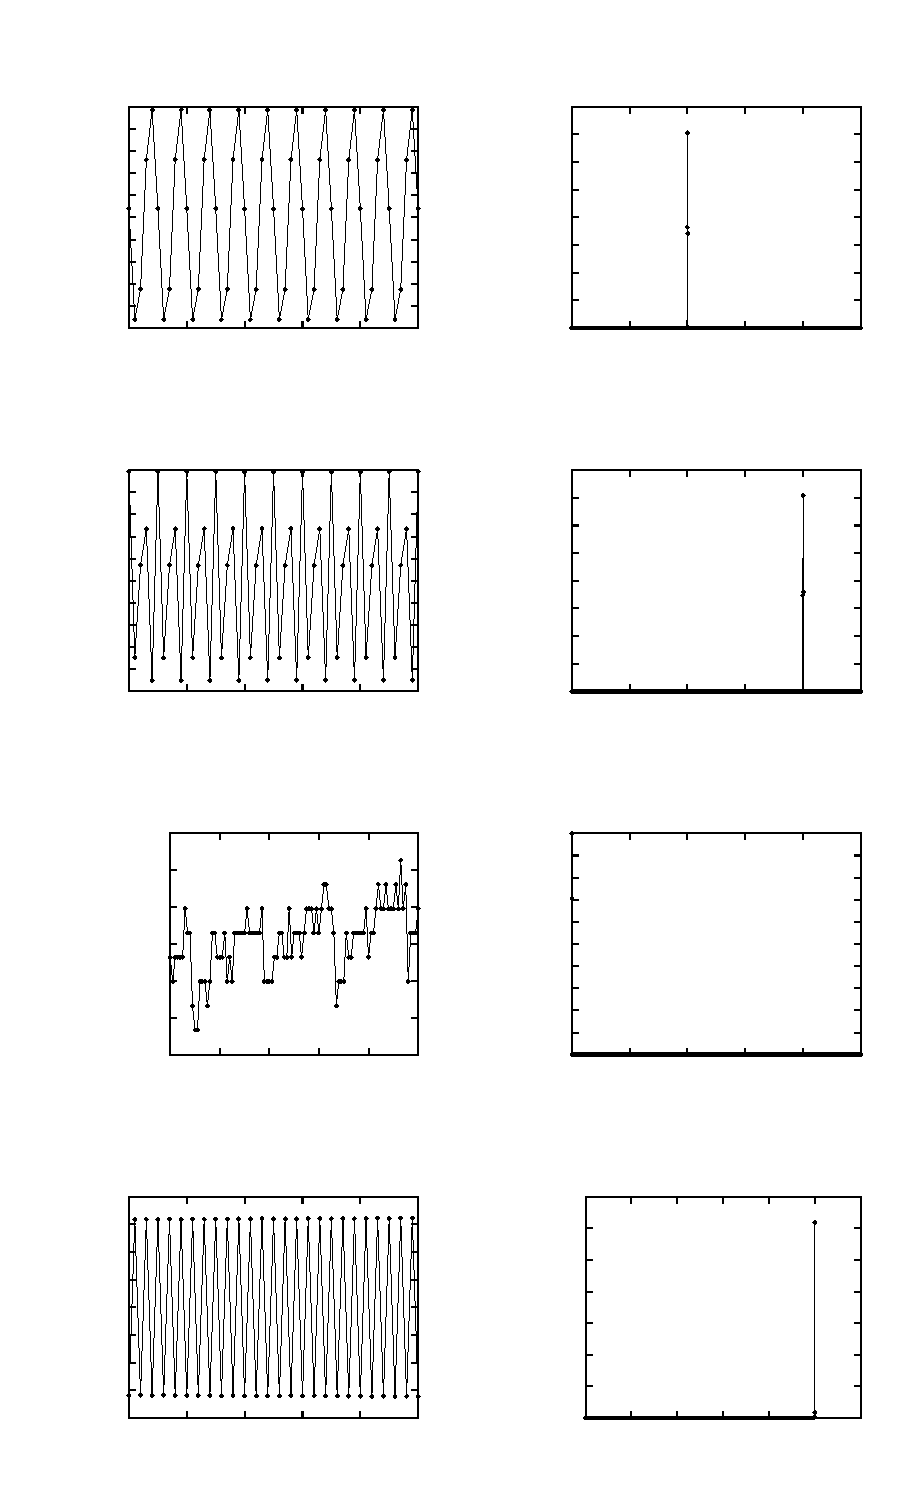
\includegraphics{2-sinus}}%
    \gplfronttext
  \end{picture}%
\endgroup
